\documentclass[letterpaper,twocolumn,10pt]{article}
\usepackage[T1]{fontenc}
\usepackage{mathptmx}
\usepackage[margin=0.75in,columnsep=0.3in]{geometry}
\usepackage{array,booktabs,graphicx,microtype,xcolor,url,amsmath}
\usepackage[hidelinks]{hyperref}
\urlstyle{same}
\usepackage[font=small,skip=4pt]{caption}
\usepackage{listings}
\lstset{basicstyle=\ttfamily\footnotesize,columns=fullflexible,frame=none,numbers=left,numberstyle=\tiny,xleftmargin=1.5em,firstnumber=auto}
\newcommand{\code}[1]{\texttt{\small #1}}
\newcommand{\hr}[1]{\texttt{\small #1}}
% Numbers used in paper.tex, each traceable to a run (docs/runs/win2-log.md).
% ST-1: results/win10-lab/ST-1/20261017T224858Z, analysis/gate.py (window 23:18:58-04:48:58Z).
\newcommand{\STaQueries}{381{,}600}
\newcommand{\STaOk}{360{,}000}
\newcommand{\STaDetErr}{21{,}600}
\newcommand{\STaPrivSlope}{0.037}
\newcommand{\STaPrivCI}{[$-0.007$, 0.082]}
\newcommand{\STaPerRead}{0.06}
\newcommand{\STaPerReadCI}{[$-0.01$, 0.14]}
\newcommand{\STaArrayReads}{3.48\,M}
% ST-2: results/win10-lab/buggy-ST-2/20261018T072639Z, analysis/gate.py (window 07:56:39-08:26:39Z).
\newcommand{\STbLeak}{140--300}
\newcommand{\STbSummary}{at $k=10$ for 1\,h (3{,}180 queries and 31{,}650 array reads in the 30-minute measurement window) the client's private bytes grew 8.5\,MB/h, i.e.\ 141.5\,B per array read (95\% CI [139.3, 143.6]), against 0.06\,B for the correct client (Table~\ref{tab:st1}); the probe's own ledger flagged 780 unreleased values. The leak grows with reads, not with connection age, and Agent A's data above show that recycling does not release it.}
% E-fault: results/win10-lab/E{0,1,2,3}-fault/, analysis/efault.py (deterministic keys excluded).
\newcommand{\EthreeErr}{59{,}995}
\newcommand{\EthreeRec}{none in 60 min}
\newcommand{\EthreeText}{Agent A's pool behaved exactly like no refresh (59{,}995 errors, no recycle): \hr{RPC\_S\_SERVER\_UNAVAILABLE} is not an outer code its health check treats as unhealthy, and at arm end its connections were 1.5\,h of 6\,h old with at most 21{,}000 of 50{,}000 queries. By its rules the first recycle would come from the query budget at about 214\,min ($k=100$) or the 6\,h age limit (production rate); we did not run that long. The refresh mechanism did not fire on the one fault that needed it.}
\newcommand{\EfaultHeadline}{a restart of the WMI service breaks every existing connection permanently; reconnecting on the error restored service within 6\,s, a 1-hour timer after 30\,min, and a replica of Agent A's pool not within the hour, because its health check does not recognise the error.}
% H (7 days, k=100): running.
\newcommand{\HNote}{A 7-day run at $k=100$ (about 300 production-days of queries per connection) is in progress and will replace this section's age bound.}
\newcommand{\HAgeNote}{; the 7-day run is in progress}


\title{\Large\bfseries Clients Rot, Connections Don't:\\ Degradation, Silent Failures and Refresh in Long-Lived WMI Connections}
\author{Author Name\\ \normalsize Affiliation}
\date{\ifdraft\small Draft v4, 2026-10-20. \authornote{Red: author input}\fi}

\raggedbottom
\begin{document}
\maketitle

\begin{abstract}
Windows management agents commonly recycle their WMI connections every few hours on the belief that long-lived connections degrade.
We test that belief with a client whose COM usage is verified on every query, which checks results against non-WMI ground truth and attributes resource use to the provider host serving each query.
On two hosts, one Windows~10-based and one Windows~11-based, one set of connections served \STaQueries{} and \STbQueries{} queries over 6\,h at 100$\times$ and \WbK{}$\times$ a production polling rate (about 25 and 12.5 production-days of queries).
Latency, median and 99th percentile, did not change with connection age on either host.
Client memory did not grow measurably on the first (\STaPrivSlope{}\,MB/h, 95\% CI \STaPrivCI{}; an upper bound near 7.5\,MB/year at the production rate); on the second it grew slowly (\STbPrivSlope{}\,MB/h \STbPrivCI{}), well below our pre-set bound (about 40\,MB/year at the production rate) and fully reclaimed when the connections closed, though whether it reaches a plateau is still open.
The degradation we could reproduce was client-induced: an unreleased \code{VARIANT} array leaks about \STtwoLeak{}\,B per read, and cross-apartment calls to the scripting objects cost about 3$\times$ the wall-clock time per collection cycle (5--8$\times$ the CPU).
\emph{Silent} failures matter more: a popular Go COM library ends enumeration without reporting the error, three of the earlier client's 23 queries fail on every poll on both architectures while logged as successes, and \code{Win32\_SystemDriver} omits a registered driver whose binary is missing, depending on the properties selected.
Fault injection shows where refresh matters: on both hosts a restart of the WMI service broke every existing connection permanently; reconnecting on the error restored service within seconds, a 1-hour timer after 30\,min, and a replica of our earlier client's pool not within the hour, because its health check does not recognise the error.
A crash of a provider host cost at most the call it was serving; the connection survived.
Agents should invest in client correctness and result verification, and reconnect on errors rather than on a clock.
\end{abstract}

\section{Introduction}
Windows Management Instrumentation (WMI) is the standard inventory and telemetry interface on Windows; endpoint agents, monitoring systems and configuration tools poll it continuously.
A widespread practice is to treat WMI connections as perishable: agents tear down and recreate their \code{IWbemServices} connections on a timer or a query budget.
The belief is documented in the tooling as well as in operations: a widely used Go WMI package warns of a ``memory bug'' and advises callers to run queries in a dedicated process and exit after a bounded number of queries~\cite{se-wmi}, and reported client leaks have been traced to unreleased COM objects rather than to connection age~\cite{zbx-8506}.
This belief is where we began.
While building esinta, our OT endpoint-telemetry agent, we saw its WMI client's memory grow, its latency creep and its calls time out, and took these for connection ageing.
We built the probe described here to test that hypothesis against our earlier client, the WMI layer of earlier esinta builds, which issues the 23 queries below and recycles every 6\,h or 50{,}000 queries, the standard refresh-on-timer rule.\authornote{provenance check: the records (evidence inventory; pull requests 69, 93, 115, 118, 164) show the earlier client is esinta's own WMI layer, not a separate client built for the test; the probe is what was built to test the hypothesis. Confirm this wording}
We expected to confirm that long-lived connections rot; instead the verified client showed the degradation was ours.
\emph{Disclosure:} the authors develop esinta commercially; the earlier client studied here and the bugs reported in it are our own, found and fixed between September and October 2026.\authornote{if the venue is double-blind, move this disclosure to the un-blinded conflict-of-interest statement, since naming esinta de-anonymises}

Whether those symptoms come from \emph{connection age} or from the \emph{client} has, to our knowledge, not been measured.
It is hard to measure: an incorrect client produces exactly these symptoms, the usual metric (memory summed over all \code{WmiPrvSE.exe} processes) mixes every WMI client on the host, and many WMI failures are silent.

We contribute (1)~a method that removes these confounders: a self-tested correct client, per-provider-host attribution, an ETW meter of foreign WMI clients, and non-WMI ground truth (\S\ref{sec:method}); (2)~evidence on two architectures that a correct client's connections do not degrade in latency, and that client memory stays small and below a pre-set bound, at accelerated query counts (\S\ref{sec:correct}); (3)~measurements of two client bugs that produce the folklore symptoms, and a catalogue of silent failures (\S\ref{sec:client}, \S\ref{sec:silent}); and (4)~a fault-injection comparison of refresh strategies with concrete guidance (\S\ref{sec:fault}, \S\ref{sec:discussion}).

\section{Background}
A client calls \code{IWbemServices} in the WMI service (\code{Winmgmt}), which dispatches each class to a provider.
In-process providers run in shared \code{WmiPrvSE.exe} host processes, one per hosting model such as NetworkService or LocalService~\cite{ms-hosting}.
WMI unloads a provider once it has been idle for its cache-control interval (\code{ClearAfter}; unloading takes ``anywhere from the interval \ldots{} to twice that interval'')~\cite{ms-unload,ms-cachecontrol}, and enforces per-host quotas on memory, threads and handles~\cite{ms-quota}.
Queries issued with the return-immediately and forward-only flags (0x30) are semisynchronous: \code{ExecQuery} returns an enumerator at once, and errors surface later from \code{IEnumWbemClassObject::Next}, which returns \hr{WBEM\_S\_FALSE} at the normal end of a result~\cite{ms-next}.
The scripting objects (\code{SWbemLocator} and relatives) are apartment-threaded: a call from another apartment is marshalled to the owning single-threaded apartment (STA)~\cite{ms-sta}, and property values arrive as \code{VARIANT}s that the caller must free with \code{VariantClear}, which frees strings and arrays~\cite{ms-variantclear}.
A client that walks a result set through the scripting objects enumerates an \code{SWbemObjectSet} via \code{IEnumVARIANT::Next}~\cite{ms-enumvariant} rather than \code{IEnumWbemClassObject::Next}; the two share the convention that \hr{S\_FALSE} with no object marks the normal end of a result.
Throughout, we distinguish the \emph{outer} \code{HRESULT} a client sees at the call boundary from the \emph{effective} error code: a failure dispatched through \code{IDispatch::Invoke} is reported to the caller as \hr{DISP\_E\_EXCEPTION} with the originating WBEM or RPC code carried in the \code{EXCEPINFO}, so a health check that inspects only the outer code can miss a connection-level fault~\cite{ms-wmierr}.

\section{Method}\label{sec:method}
\paragraph{A correct client.}
The probe (Go, \texttt{go-ole}) gives every connection its own OS thread initialised as an STA, and makes every COM call for that connection, including release, on that thread.
Every \code{VARIANT} is cleared exactly once; a ledger counts acquisitions and releases per query and flags outstanding or double releases.
Enumeration uses a strict loop: \hr{S\_OK} yields an item, \hr{S\_FALSE} with no item ends the result, and any other code is an error recorded with its \code{HRESULT}, WBEM code and the operation that failed.
A query that exceeds its deadline is abandoned on the caller's side and its row is written when WMI eventually answers.

\paragraph{Workload.}
The catalogue reproduces the 23 queries of our earlier client verbatim (processes, services, drivers, event logs, firewall, Defender, WMI subscriptions, scheduled tasks, Device Guard, TPM, BitLocker), each at its production rate.
A query runs only where its namespace exists: on the Windows~10-based host 22 queries in 7 namespaces (BitLocker's namespace is absent; 636 queries/h), on the Windows~11-based host all 23 in 8 namespaces (648 queries/h).
The probe holds three connections to \code{root\textbackslash cimv2} and one to each other namespace (9 and 10 connections).
An acceleration factor $k$ multiplies every rate.
A pre-flight calibration on each host (10-minute steps, $k\in\{1,5,10,20,50,100\}$) measured probe-induced CPU (probe + all provider hosts + \code{Winmgmt}, as a percentage of the 2-vCPU host) of \WaRamp{} on the Windows~10-based host and \WbRamp{} on the Windows~11-based host, with no dropped queries; $k_H$, the largest $k$ within a 40\% budget, is 100 (the top of the ramp) and \WbK{}.
The two hosts' virtual CPU models differ, so absolute latency and CPU are compared within a host, not across hosts.

\paragraph{Attribution and isolation.}
Every 10\,s the probe samples itself, the \code{Winmgmt} service host (PID from the service control manager) and each \code{WmiPrvSE} by PID and creation time, labelled with its account and the provider DLLs it has loaded; this maps each queried class to the host serving it.
Nothing here uses WMI.
The class-to-host map was the same on both hosts: the CIMWin32, event-log, firewall, scheduled-task, Device Guard, TPM and (where present) BitLocker providers share the NetworkService host, and Defender's provider runs in the LocalService host.
A real-time ETW session on \code{Microsoft-Windows-WMI-Activity}~\cite{ms-tracing} counts operation starts by client PID, so foreign WMI clients are observed rather than assumed absent: in a 60-minute idle baseline it counted \WaIdle{} and \WbIdle{} foreign operations per hour on the two hosts, against a ceiling of 60/h fixed in the pre-registered design (one foreign operation per minute on average, under 0.2\% of the probe's own queries at $k_H$): a meter window above it is flagged, and an arm with more than 10\% of its windows flagged is invalid.
During the arms the session was duty-cycled, one minute in fifteen, to limit its own overhead, so foreign activity is sampled; flagged windows are reported in Section~\ref{sec:discussion}.
Because service-host grouping differs across editions and memory sizes~\cite{ms-svchost}, we read from the service control manager whether \code{Winmgmt} runs in its own \code{svchost.exe} or shares one: on both hosts it ran alone in its own.
We found that \code{tasklist.exe}, the CIM cmdlets and PowerShell remoting all issue WMI calls; host inspection during runs was restricted to tools measured at zero WMI operations.

\paragraph{Ground truth.}
Results are compared with non-WMI sources taken immediately before and after each query: the process list (\code{NtQuerySystemInformation}), the service control manager, and invariants captured at the start.
Five silent classes are counted: S1 impossible-empty, S2 truncated (a key present in both truth snapshots is missing), S3 enumeration ended by an error (what a lenient loop would report as success), S4 partial objects, S5 content mismatch.

\paragraph{Testbed and statistics.}
Two virtual machines with 2 vCPU each, one Windows~10-based (4\,GB) and one Windows~11-based (\WbRAM{}), both with Defender real-time protection on and no other WMI-heavy software.
Both hosts ran the same probe build and analysis code.
Growth is the OLS slope of 10\,s samples after a 30-minute warm-up with Newey--West standard errors (15-minute lag window)~\cite{newey-west}.
Pass criteria were fixed before the runs, in a timestamped commit of the design (\code{7f3cbb9}, 2026-10-16; the analysis implementing them, \code{3cfbca5}, is unchanged since 2026-10-17) \authornote{archive the repository publicly so these timestamps are verifiable}: client private-byte slope $<1$\,MB/h and $<3$\,B per array read (upper 95\% bound), handle range $\le 50$, and $\le 5$\,MB retained after a 1-hour release test.
Memory figures use MB $=10^6$ bytes throughout.

\section{A correct client's connections do not degrade}\label{sec:correct}
\begin{table}[t]\centering\footnotesize\setlength{\tabcolsep}{3pt}
\caption{ST-1: one set of connections, strategy \emph{none}, 6\,h, on each host. All slopes are over the same 5.5-hour window (after the 30-minute warm-up) and are net over it; how growth is distributed within the window is given in the text. CIs are 95\%, HAC. Memory in MB $=10^6$\,B.}\label{tab:st1}
\begin{tabular}{@{}lrr@{}}\toprule
& Win~10-based & Win~11-based\\\midrule
$k$ (production-days of queries) & 100 (25) & \WbK{} (12.5)\\
Queries & \STaQueries{} & \STbQueries{}\\
\quad ok & \STaOk{} & \STbOk{}\\
\quad deterministic error / abandoned & \STaDetErr{} / 0 & \STbDetErr{} / 0\\
Silent failures above truth baseline & 0 & 0\\
Client private bytes (MB/h) & \STaPrivSlope{} & \STbPrivSlope{}\\
& \STaPrivCI{} & \STbPrivCI{}\\
\quad per array read (B) & \STaPerRead{} & \STbPerRead{}\\
& \STaPerReadCI{} & \STbPerReadCI{}\\
\quad array reads & \STaArrayReads{} & \STbArrayReads{}\\
Client handles: range & 17 & 9\\
Retained after 1\,h release (MB) & \STaRelease{} & \STbRelease{}\\
NetworkService host (MB/h) & 0.085 & 0.267\\
& [0.066, 0.103] & [0.142, 0.392]\\
LocalService host (MB/h) & 0.036 & 0.090\\
& [0.001, 0.071] & [0.057, 0.122]\\
Winmgmt host (MB/h) & $-0.020$ & 0.034\\
& [$-0.043$, 0.003] & [0.016, 0.052]\\
Latency p99, last vs.\ first hour$^a$ & $-1.1$ to $+0.4$\% & $-2.2$ to $+0.8$\%\\
Recycles; induced CPU & 0; 30.2\% & 0; 24.8\%\\\bottomrule
\multicolumn{3}{@{}p{0.92\columnwidth}}{$^a$ range over the query keys with median latency above 100\,ms (six and seven keys).}
\end{tabular}
\end{table}
The self-test arm (strategy \emph{none}: one set of connections held open for the whole run, with the probe's per-query COM ledger active) doubles as our longest correct-client run on each host (Table~\ref{tab:st1}).
At $k=100$ its 6 hours carry the query count of about 25 days at the production rate (12.5 days at $k=\WbK{}$).
This accelerates the \emph{count} of queries, not the age of the connection and not the provider lifecycle: at these rates the providers never go idle long enough to unload, so the arm contains none of the unload/reload cycles a production client sees every few minutes (below).
All client invariants held on every query on both hosts (correct apartment, no outstanding, double or leaked \code{VARIANT}s, no panics), and both passed the pre-set criteria.

\paragraph{Windows~10-based host.}
Client memory did not grow measurably.
If growth tracks queries, we can rule out at the production rate a client-side leak larger than about 0.86\,kB/h (roughly 7.5\,MB/year) at 95\% confidence.
Median latency per query key stayed flat across connection age, from about 2\,ms (repository classes) to 230\,ms (\code{MSFT\_NetFirewallRule}, 260 rows; first to last hour of the window $-2$\%).
The tails were as flat: for the six keys with medians above 100\,ms, the 95th and 99th percentiles moved by at most 1.6\% from the first to the last hour, no key's 99th percentile rose by more than 1.9\,ms, and no successful query took longer than 363\,ms against a 30\,s deadline (none was abandoned).
The \code{Winmgmt} host was flat ($-0.020$\,MB/h [$-0.043$, 0.003]).
The provider hosts grew mostly early: by thirds of the window, the LocalService host 0.19, 0.01 and $-0.03$\,MB/h, and the NetworkService host, serving six providers, 0.13, 0.07 and 0.02\,MB/h [$-0.09$, 0.13] (0.085\,MB/h [0.066, 0.103] over the window, about 0.5\,MB in 5.5\,h).
Six hours cannot distinguish a plateau from slow growth there; the 7-day run will.
The single client handle step (339 to 347) coincides with one additional Go runtime thread and is flat before and after.
\HNote{}

\paragraph{Windows~11-based host.}
Latency was again flat with connection age: first-to-last-hour medians moved by less than 1\% for \code{MSFT\_NetFirewallRule} (648\,ms, 492 rows), \code{Win32\_SystemDriver} (272\,ms) and \code{Win32\_Service} (191\,ms), and by 2\% for the full process list (167 to 170\,ms).
For the seven keys with medians above 100\,ms the 95th and 99th percentiles moved by at most 2.6\%, no key's 99th percentile rose by more than 3.2\,ms, and no successful query took longer than 940\,ms against a 30\,s deadline (none was abandoned).
The provider hosts and the \code{Winmgmt} host grew modestly over the window (Table~\ref{tab:st1}), most of the rise in the first third: by thirds, the NetworkService host, now with seven providers, 1.37, $-0.19$ and $-0.06$\,MB/h (30-minute medians 13.1 to 14.7\,MB), the LocalService host 0.27, 0.09 and 0.02, and the \code{Winmgmt} host 0.13, 0.03 and 0.01\,MB/h, the last two thirds' intervals all including zero.
The client's private bytes, however, grew \STbPrivSlope{}\,MB/h \STbPrivCI{} (\STbPerRead{}\,B per array read): distinguishable from zero, but 4.3$\times$ below our pre-set bound and small in absolute terms (27.5 to 29.0\,MB over the arm, and about 4.6\,kB/h, or 40\,MB/year, at the production rate if it tracks queries).
The growth was uneven across the window (by thirds 0.42, 0.04 and 0.40\,MB/h), so these 6 hours cannot tell whether it continues linearly or approaches a plateau.
The Go heap was flat ($-0.010$\,MB/h [$-0.041$, 0.021]), locating the growth in native memory, and it was fully reclaimed when the connections were released: at the end of the release test the client was 0.90\,MB below its post-warm-up level.
The ledger accounts for \code{VARIANT}s, so its clean result rules out a leaked \code{SAFEARRAY} or \code{BSTR}, not all per-connection native allocation; the likeliest source is client-side object-cache or per-connection COM/RPC proxy state, which we did not instrument.
This is consistent with memory held on behalf of open connections rather than an unbounded leak; the two are separable only by whether the growth plateaus, which a longer run on this host will decide (Figure~\ref{fig:client}).
Because closing a connection reclaims this memory, the result can be read as an argument for periodic reconnection.
It is a weak one.
Even if the growth is linear in queries and never levels off, at the production rate it amounts to about 3.3\,MB per month of connection age, so reconnecting monthly would bound it there; our earlier client's 6-hour cycle reconnects about 120 times as often, and Section~\ref{sec:fault} shows that a timer recovers from the one fault that does break a connection only when it next fires (30\,min in our runs), against seconds for reconnecting on the error.
\authornote{plateau run: a Windows~11-based strategy-\emph{none} run of 48--72\,h is proposed after the current battery; until then the paragraph above is the case}

\begin{figure}[t]\centering
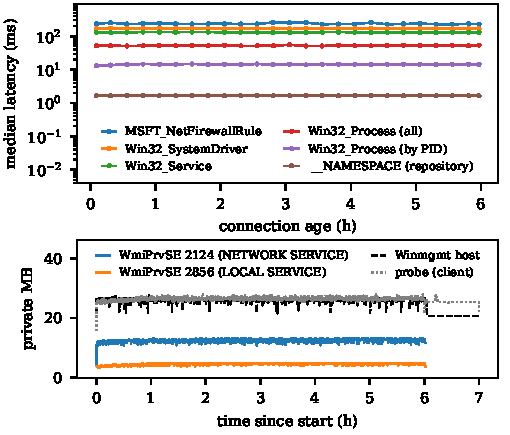
\includegraphics[width=\columnwidth]{fig-st1.pdf}
\caption{ST-1, Windows~10-based host. Top: median latency per 15-minute window against connection age for six query keys. Bottom: private bytes of the two provider hosts (labelled by account and number of providers; the providers are listed in Section~\ref{sec:method}), the Winmgmt host and the client; connections were released at 6\,h. The Windows~11-based client is in Figure~\ref{fig:client}.}\label{fig:st1}
\end{figure}

\begin{figure}[t]\centering
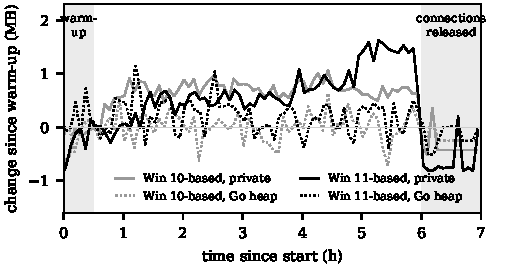
\includegraphics[width=\columnwidth]{fig-client.pdf}
\caption{Client memory in ST-1 on both hosts: change in private bytes (solid) and Go heap (dotted) since the end of warm-up, 5-minute medians. Connections were released at 6\,h.}\label{fig:client}
\end{figure}

\paragraph{Providers reload anyway.}
On both hosts, read from the \code{\_\_CacheControl} and \code{\_\_ProviderHostQuotaConfiguration} instances, \code{ClearAfter} is 30\,s (15\,s for event sinks) and the provider-host quotas are identical (512\,MB per host, 1\,GB for all hosts, 4{,}096 handles, 256 threads, 32 processes): neither is tuned per architecture.
At the production rate ($k=1$) most classes are queried less often than that, and on the Windows~10-based host the WMI-Activity log showed six providers reloading every 1--2 minutes \emph{inside} one long-lived host PID (event 5857 within 10 minutes); the Defender provider's host itself was replaced, and idle hosts exited 60--65\,s after release (60\,s on the Windows~11-based host).
A production client thus gets a free refresh of provider state every few minutes; only its connection and the WMI service age.

\section{What degrades is the client}\label{sec:client}
\paragraph{Unreleased arrays (our earlier client, pull request 115).}
Property values read through \code{Properties\_} that were never passed to \code{VariantClear} leak their \code{SAFEARRAY}s.
In long soak runs of the earlier client this was steady memory growth (+1.45\,MB/h over 13.5\,h on a Windows~10 VM, +2.29\,MB/h over 20\,h on a laptop) that scaled with the firewall collector's frequency (+8.8\,$\pm$\,0.6\,MB/h at 60\,s, +0.44\,$\pm$\,0.52 after the fix) and that \emph{recycling did not cure} (2.5\,MB/h with recycling working): the leak is in the client.
Our positive control re-enables the bug in the probe.
On the Windows~10-based host at $k=10$ for 1\,h (3{,}180 queries and 31{,}650 array reads in the 30-minute measurement window) the client's private bytes grew 8.97\,MB/h [8.82, 9.10], i.e.\ 141.5\,B per array read (95\% CI [139.3, 143.6]), against 0.06\,B for the correct client (Table~\ref{tab:st1}); the probe's ledger flagged 780 \code{VARIANT} values acquired and never released in the window (about 5.7\,kB per retained value, consistent with the firewall-rule \code{SAFEARRAY}s).
On the Windows~11-based host we ran the control at two rates, $k=5$ and $k=10$: per array read the leak was \STtwoWbKfive{}\,B \STtwoWbKfiveCI{} and \STtwoWbKten{}\,B \STtwoWbKtenCI{}, with overlapping CIs at the two rates and within 4\% of the Windows~10-based value, while the hourly growth doubled (\STtwoWbRateFive{} to \STtwoWbRateTen{}\,MB/h).
The leak therefore tracks reads, not connection age, in our controlled runs as well as in the earlier client's frequency sweep, and recycling did not release it.

\paragraph{Cross-apartment calls (pull request 118).}
Our earlier client called the apartment-threaded scripting objects from multi-threaded-apartment goroutines, so COM marshalled every call into a single host STA (confirmed in debugger stacks).
Moving each connection to its own STA cut the wall-clock time per collection cycle about 3$\times$ (process poll 1.31--1.40\,s to 0.42--0.44\,s; firewall rules 8.5\,s to 2.8\,s) and steady-state CPU on a busy 16-CPU laptop from 28.3\% to 3.5--3.9\% of a core (a 5--8$\times$ reduction), eliminating 1{,}490 abandoned calls in 69\,h ($\approx$21/h).
On a quiet 2-vCPU VM the same bug cost 5.0\% vs 0.9\% and caused no abandoned calls: the symptom scales with host load, which makes it look like ageing on busy machines.
This cost is specific to clients that drive the apartment-threaded scripting objects across apartments; native \code{IWbemServices} clients and clients on the newer Management Infrastructure (MI) API~\cite{ms-mi} do not marshal through a single STA and would not show it.\authornote{verified: 115 and 118 are merged pull requests (2026-09-25 and 2026-09-28) in our esinta repository, which is private, so readers cannot open them; decide whether to cite them as private, or archive their descriptions and measurements with the artifact and cite that}

\section{Silent failures}\label{sec:silent}
\paragraph{A library that swallows errors.}
In \texttt{go-ole} v1.3.0~\cite{go-ole}, \code{oleutil.ForEach} (\code{oleutil.go}, lines 118--126) enumerates an object's \code{\_NewEnum} through \code{IEnumVARIANT} and loops while the number of items returned is positive:
\begin{lstlisting}[firstnumber=118]
for item, length, err := enum.Next(1); length > 0;
    item, length, err = enum.Next(1) {
  if err != nil { return err }
  ...
}
return nil
\end{lstlisting}
When \code{Next} fails with zero items, the loop condition is false, the error is never inspected and the function returns \code{nil}.
The same gap truncates a result silently when \code{Next} fails after some items have been returned: those items are delivered, the terminating error is dropped, and the caller sees a short but ``successful'' enumeration.
On both hosts, \code{SELECT * FROM} a non-existent class fails only at \code{Next} with \hr{WBEM\_E\_INVALID\_CLASS} (0x80041010); \code{ForEach} reports success with 0 items, while our strict loop records the error.

\paragraph{Production queries that never worked.}
Three of the earlier client's 23 queries fail at \code{Next} on every call, with the same codes on both architectures (Table~\ref{tab:silent}).
On the Windows~10-based host, in the 7\,h before we stopped the client there to begin this study, WMI-Activity recorded 84 \hr{5858} errors for each, while the client's own result log recorded a 0-row, 0\,ms success at each of their positions in every cycle (the log has no query text, so attribution is by position).
From the client's code, the consequences are concrete: the firewall collector records no application path, non-standard event consumers are missing from the persistence inventory, and scheduled tasks lack last-run and next-run times.
Each was a plausible-looking query.
\code{Name} is not a property of the abstract \code{\_\_EventConsumer} base class (which has \code{CreatorSID}, \code{MachineName} and \code{MaximumQueueSize}); it appears only on the five derived consumer classes~\cite{ms-eventconsumer}.
\code{MSFT\_NetApplicationFilter} exposes \code{AppPath} and \code{Package} but no \code{Program} (class definition read on-host with \code{Get-CimClass}); ``Program'' is the name of the \code{Set-NetFirewallApplicationFilter} cmdlet parameter~\cite{ms-setfwapp}, the likely origin of the mistake.
\code{MSFT\_ScheduledTaskInfo} is not a WMI class; the per-task run times are exposed through \code{MSFT\_TaskDynamicInfo} (\code{LastRunTime}, \code{NextRunTime}, \code{LastTaskResult}, \code{NumberOfMissedRuns}; class definition read on-host with \code{Get-CimClass})~\cite{ms-taskinfo}.

\begin{table}[t]\centering\small
\caption{Silent failures. All return success to a lenient client. Codes are the strict loop's, at \code{Next}, on every call.}\label{tab:silent}
\begin{tabular}{@{}>{\raggedright\arraybackslash}p{0.35\columnwidth}>{\raggedright\arraybackslash}p{0.27\columnwidth}>{\raggedright\arraybackslash}p{0.27\columnwidth}@{}}\toprule
Query / class & Win~10-based & Win~11-based\\\midrule
\code{SELECT Name FROM \_\_EventConsumer} & \hr{0x80041017} & \hr{0x80041017}\\
\code{SELECT InstanceID, Program, Package FROM MSFT\_Net\allowbreak{}ApplicationFilter} & \hr{0x80041017} & \hr{0x80041017}\\
\code{\ldots{} FROM MSFT\_Scheduled\allowbreak{}TaskInfo} & \hr{0x80041010} & \hr{0x80041010}\\
\code{Win32\_SystemDriver} with any configuration property (or \code{*}) & 333 of 334; \code{vwifibus} (binary absent) omitted & 384 of 384 (no driver lacks its binary)\\\bottomrule
\end{tabular}
\end{table}

\begin{table*}[t]\centering\small
\caption{E-fault, 90\,min per arm. Errors caused by the host kill and by the Winmgmt restart (the 60\,min after it holds 60{,}000 and 30{,}600 queries at the two hosts' rates); a call in flight when a fault began is counted with that fault (Windows~11-based host only: one call at each kill, two or three at each restart); recovery is the time until every connection that failed has answered again.}\label{tab:efault}
\begin{tabular}{@{}llrrrrrr@{}}\toprule
& & \multicolumn{3}{c}{Windows~10-based, $k=100$} & \multicolumn{3}{c}{Windows~11-based, $k=\WbK{}$}\\\cmidrule(lr){3-5}\cmidrule(l){6-8}
Arm & Strategy & kill errors & restart errors & recovery & kill errors & restart errors & recovery\\\midrule
E0 & none & 0 & 59{,}995 & none in 60 min & \EbKill{} & \EbZeroErr{} & \EbZeroRec{}\\
E1 & timed (1\,h) & 0 & 30{,}002 & 1{,}804.5\,s & \EbKill{} & \EbOneErr{} & \EbOneRec{}\\
E2 & adaptive & 0 & 8 & 6.0\,s & \EbKill{} & \EbTwoErr{} & \EbTwoRec{}\\
E3 & Earlier-client pool & 0 & \EthreeErr{} & \EthreeRec{} & \EbKill{} & \EbThreeErr{} & \EbThreeRec{}\\\bottomrule
\end{tabular}
\end{table*}

\paragraph{A provider that drops rows.}
On the Windows~10-based host \code{Win32\_SystemDriver} returned 333 drivers whenever the query selected any configuration property (\code{DisplayName}, \code{PathName}, \code{StartMode}, \code{StartName}, \code{ServiceType}, \code{Description}, or \code{*}), and 334 for \code{SELECT Name} or \code{SELECT Name, State}.
The missing driver, \code{vwifibus}, is registered with the service control manager but its image path points to a file that does not exist.
No error is returned at any layer; only the comparison with the service control manager reveals it.
A provider might reasonably omit a driver whose image cannot be read; what makes this a silent failure is that the row count depends on the projection---present for \code{SELECT Name}, absent once any configuration property is requested---with no error or other signal at any layer.
On the Windows~11-based host the same driver is registered with its binary present in the driver store, and \code{Win32\_SystemDriver} returned all 384 registered drivers for every selection.
The omission therefore depends on host state, a registered driver whose binary is missing, which is common after driver removal, rather than on the Windows architecture.
Because it is deterministic, we treat it as a per-key truth baseline and count S2 only above it.

\paragraph{Races are not failures.}
In 19{,}716 calibration queries the only other flags were three scheduled-task counts one short as the count changed and one process that exited during its query: timing, not WMI, separable only by bracketing truth before and after each query.

\section{Fault recovery and refresh}\label{sec:fault}
If connections do not age, refresh is only worth its cost as recovery from faults.
On each host we ran four 90-minute arms back to back ($k=k_H$, fresh connections each), one per strategy: \emph{none} (E0); \emph{timed}, redial every connection after 1\,h (E1); \emph{adaptive}, retire a connection when a failed call's effective error code is connection-level and redial at its next query (E2); and a replica of our earlier client's \emph{pool}, which recycles at 6\,h, 50{,}000 queries or 5\,min idle, or when the outer \code{HRESULT} maps to access denied, transport failure, ``not available'' or COM not initialised (E3; rules copied from the earlier client's source).
At 15\,min we killed the \code{WmiPrvSE} host serving \code{Win32\_Process} and its co-hosted providers; at 30\,min we restarted \code{Winmgmt} and its running dependent services through the service control manager (1.9\,s in total on the Windows~10-based host, which had two running dependents; 0.2--0.4\,s on the Windows~11-based host, which had none).
The three deterministically failing keys are excluded.

\paragraph{A provider-host crash cost at most the call in flight.}
On the Windows~10-based host each of the four kills landed between queries and no query failed: the connection is to \code{Winmgmt}, which had a replacement host with the same providers running 31\,ms later (E0), and the 99th-percentile latency in the following 30\,s was unchanged (225 vs.\ 231\,ms before).
On the Windows~11-based host, where queries take longer, each kill landed while two calls served by the killed host were in flight, at the same point of the schedule in all four arms.
A firewall-address query that had started 31--34\,ms earlier and was still waiting for its first object failed about 10\,ms after the kill, at \code{IEnumVARIANT::Next}, with \hr{RPC\_S\_CALL\_FAILED} (0x800706BE); this agrees with Microsoft's guidance that when WMI stops a host for a quota violation the query it is serving fails~\cite{ms-quota-guide}.
A driver query that started about 245\,ms earlier and was already returning rows completed with all 384 drivers, matching the service control manager.
In both cases the connection was unaffected: under no refresh, the timer and the pool the next query on it succeeded and no other query failed before the service restart 15\,min later, and the 99th-percentile latency was unchanged (687 vs.\ 692\,ms before, E0).
The adaptive client treats \hr{RPC\_S\_CALL\_FAILED} as connection-level, so it retired the healthy connection and redialled in 7.8\,ms.
The failure surfaces at \code{Next}, the call whose result the \code{ForEach} helper of Section~\ref{sec:silent} discards, so a client using it would have recorded an empty result as a success.
These are four kills at one offset into a call, not a map of every phase of a call.
\authornote{a kill via a lowered \code{MemoryPerHost} quota was not run; drop or schedule}

\paragraph{A service restart is permanent.}
After \code{Winmgmt} restarted, every call on every existing connection failed with \hr{RPC\_S\_SERVER\_UNAVAILABLE} (0x800706BA) and none recovered on its own (Windows~10-based E0: 59{,}995 of 60{,}000; the 5 successes were calls issued in the 175\,ms before the service stopped; Windows~11-based E0: all \EbZeroErr{}, including three calls in flight when the restart began, which failed with \hr{RPC\_E\_DISCONNECTED} (0x80010108) or \hr{RPC\_S\_CALL\_FAILED}).
The timed strategy was down until its timer fired, 30 minutes later; an outage of up to one refresh interval is inherent to it.
This is not peculiar to our client: Microsoft documents that its Configuration Manager client (\code{CcmExec}) is left non-functional after the WMI service is restarted, because WMI cancels outstanding requests and does not re-establish them, and recovers only when a periodic health check restarts the client~\cite{ms-ccmexec}.
The adaptive client lost exactly one query per connection: each of its 9 connections on the Windows~10-based host failed once, was retired, redialled in 1--6\,ms, and its next scheduled query succeeded; Table~\ref{tab:efault} counts 8 because one of the nine failures fell on an excluded deterministic key.
On the Windows~11-based host all 10 connections failed once (two on calls in flight when the restart began) and redialled in 1--36\,ms.
The recovery time, 6.0 and 11.5\,s, is the query interval of the least-busy namespace at each host's $k_H$ and would be one production polling interval at $k=1$.
Our earlier client's pool behaved exactly like no refresh on both hosts (59{,}995 and \EbThreeErr{} errors, no recycle): \hr{RPC\_S\_SERVER\_UNAVAILABLE} is not an outer code its health check treats as unhealthy, and at arm end its connections were 1.5\,h of 6\,h old with at most 21{,}000 (10{,}500 on the Windows~11-based host) of 50{,}000 queries.
By its rules the first recycle would come from the query budget at about 214\,min at $k=100$, from the 6\,h age limit at $k=50$ and at the production rate; we did not run that long.
The refresh mechanism did not fire on the one fault that needed it, on either host.

\section{Discussion}\label{sec:discussion}
\paragraph{Guidance.}
(1)~Make the client correct first: one STA per connection, all COM calls on it, every \code{VARIANT} cleared, and a test that runs a few hundred thousand queries and checks for growth; timed recycling hides neither of the bugs above.
(2)~Never let an enumeration end without inspecting the last \code{HRESULT}; audit libraries for this pattern.
(3)~Validate each query once at start-up and verify results against an independent source where one exists; ``0 rows'' is a claim, not a fact.
(4)~Reconnect on connection-level errors by inspecting the effective error code, not only the outer \code{HRESULT}; test the health check by restarting \code{Winmgmt}.
In our fault injection the service restart produced \hr{RPC\_S\_SERVER\_UNAVAILABLE} (observed); a robust health check should additionally treat \hr{WBEM\_E\_TRANSPORT\_FAILURE} and \hr{WBEM\_E\_NOT\_AVAILABLE} as connection-level (documented~\cite{ms-wmierr}, not observed here), and \hr{RPC\_E\_DISCONNECTED} (observed on calls in flight when the service stopped).
\hr{RPC\_S\_CALL\_FAILED} from a crashed provider host left the connection usable; retiring on it costs one redial.
A timer adds churn and leaves an outage of up to one interval.
(5)~Do not attribute \code{WmiPrvSE} growth to your client without per-host attribution and a foreign-client meter.

\paragraph{Threats to validity.}
Two hosts, one per architecture, and one workload; each fault was injected once per strategy and host, so the fault results are existence proofs of a strategy's behaviour, not rates.
The two hosts also differ in acceleration (the Windows~10-based ran at $k=100$, the Windows~11-based at $k=\WbK{}$, forced by the 40\% CPU budget), in RAM and in CPU model, so architecture, rate and hardware move together; the between-host difference in client memory growth cannot be attributed to the operating system alone. The CPU model does not explain the lower rate: the probe's induced CPU per query on the Windows~11-based host was about twice that on the Windows~10-based host, and stayed so when we re-calibrated it with the same CPU model as the Windows~10-based host (\WcRamp{} over the six ramp steps, so $k_H=\WcK{}$ again).
Accelerating the query rate tests count, not age, and not the provider unload/reload cycle, which at $k_H$ does not occur: our longest correct-client connections are 6\,h old\HAgeNote{} on the Windows~10-based host only.
On the Windows~11-based host the client's connection-held memory grew throughout the 6\,h arm; whether it levels off is open.
The ETW meter ran one minute in fifteen in every arm, so foreign activity is sampled, and the pre-registered rule (an arm is invalid when more than 10\% of its windows exceed 60 foreign operations per hour) was met by every self-test and client-bug arm but not by six of the eight fault arms. In the self-test and client-bug arms one window was flagged, in the Windows~10-based ST-1 (1 of 24: 6 operations from a system service, most likely the Windows Update service by timing). Each of the six fault arms had one flagged window of six. On the Windows~10-based host it was, in all four arms, the window containing the service restart: 38 operations in the 10\,s after it, from two system service hosts querying \code{HNet\_ConnectionProperties} and \code{Win32\_ComputerSystemProduct}, consistent with the two dependent services the restart also restarts (not confirmed by PID). On the Windows~11-based host a network-service host polled network-adapter classes about once per second for a minute, in E0 in the minute that began with the provider-host kill (60 operations) and in E3 at 61\,min (22); E1 and E2 saw none. The fault arms' outcomes are the error codes and recovery times of our own connections; we report all eight arms and declare this as a deviation from the pre-registration.\authornote{decision: keep the six fault arms as a declared deviation (as drafted), exclude fault-induced windows from the rule post hoc and say so, or present the fault arms as exploratory; the Windows~10-based restart window is induced by our own fault, the Windows~11-based E3 window is not}
The earlier client's degradation numbers come from before/after comparisons of single changes across our soak-test hosts (a VM and a laptop).
Our no-degradation result is for a client whose COM usage is correct on this provider set; providers themselves can leak, as in a documented \code{WmiPrvSE} user-profile case~\cite{ms-kb2832248}, which per-host attribution (guidance 5) is designed to separate from client growth.
Older and server-only architectures, and further client builds, remain future work.

\paragraph{Related work.}
Microsoft documents the mechanisms we rely on: provider hosting and unloading~\cite{ms-hosting,ms-unload}, quotas~\cite{ms-quota}, enumeration semantics~\cite{ms-next} and COM apartment rules~\cite{ms-sta}.
The newer Management Infrastructure (MI) API~\cite{ms-mi} is the client surface the CIM cmdlets use and a natural target for replication; our findings here are for a COM/scripting client, and whether they transfer to MI and to native \code{IWbemServices} clients is open.
We are not aware of published measurements of WMI connection ageing under a verified-correct client, nor of a catalogue of WMI silent failures; we welcome pointers.

\section{Conclusion}
Long-lived WMI connections, used correctly, did not degrade in latency, median or tail, on either architecture; the provider hosts and the WMI service grew by less than 2\,MB over the 5.5-hour measurement window, mostly in its first third, and the client by at most 1.5\,MB, all of it returned when the connections closed; the symptoms we could reproduce were produced by the client, and the costliest failures were silent.
Refresh is a recovery mechanism, best driven by errors.
The probe, catalogue and analysis code are available from the authors \authornote{replace with a public repository URL and an artifact DOI}.

\footnotesize\raggedright
\begin{thebibliography}{22}\setlength{\itemsep}{0pt}
\bibitem{ms-hosting} Microsoft. \emph{Provider Hosting and Security}. \url{https://learn.microsoft.com/en-us/windows/win32/wmisdk/provider-hosting-and-security}
\bibitem{ms-unload} Microsoft. \emph{Unloading a Provider}. \url{https://learn.microsoft.com/en-us/windows/win32/wmisdk/unloading-a-provider}
\bibitem{ms-cachecontrol} Microsoft. \emph{\_\_CacheControl class}. \url{https://learn.microsoft.com/en-us/windows/win32/wmisdk/--cachecontrol}
\bibitem{ms-quota} Microsoft. \emph{\_\_ProviderHostQuotaConfiguration class}. \url{https://learn.microsoft.com/en-us/windows/win32/wmisdk/--providerhostquotaconfiguration}
\bibitem{ms-next} Microsoft. \emph{IEnumWbemClassObject::Next}. \url{https://learn.microsoft.com/en-us/windows/win32/api/wbemcli/nf-wbemcli-ienumwbemclassobject-next}
\bibitem{ms-sta} Microsoft. \emph{Single-Threaded Apartments}. \url{https://learn.microsoft.com/en-us/windows/win32/com/single-threaded-apartments}
\bibitem{ms-variantclear} Microsoft. \emph{VariantClear function}. \url{https://learn.microsoft.com/en-us/windows/win32/api/oleauto/nf-oleauto-variantclear}
\bibitem{ms-tracing} Microsoft. \emph{Tracing WMI Activity}. \url{https://learn.microsoft.com/en-us/windows/win32/wmisdk/tracing-wmi-activity}
\bibitem{go-ole} go-ole contributors. \emph{go-ole v1.3.0, oleutil/oleutil.go}. \url{https://github.com/go-ole/go-ole/blob/v1.3.0/oleutil/oleutil.go}
\bibitem{newey-west} W.~K. Newey and K.~D. West. A simple, positive semi-definite, heteroskedasticity and autocorrelation consistent covariance matrix. \emph{Econometrica}, 55(3):703--708, 1987.
\bibitem{se-wmi} StackExchange. \emph{wmi: Go WMI package}, README warning on the memory bug. \url{https://github.com/StackExchange/wmi}
\bibitem{zbx-8506} Zabbix. \emph{ZBX-8506: wmi.get on Windows agent causes memory leak (unreleased pclsObj)}. \url{https://support.zabbix.com/browse/ZBX-8506}
\bibitem{ms-ccmexec} Microsoft. \emph{SMS Agent Host service isn't automatically restarted after the WMI service restarts}. \url{https://learn.microsoft.com/en-us/troubleshoot/mem/configmgr/client-management/sms-agent-host-not-automatically-restarted}
\bibitem{ms-quota-guide} Microsoft. \emph{Scenario guide: troubleshoot WmiPrvSE quota-exceeded issues}. \url{https://learn.microsoft.com/en-us/troubleshoot/windows-server/system-management-components/scenario-guide-troubleshoot-wmiprvse-quota-exceeded-issues}
\bibitem{ms-kb2832248} Microsoft. \emph{Memory leak occurs in the Wmiprvse.exe process in Windows~7 or Windows Server 2008~R2} (KB2832248). \url{https://support.microsoft.com/en-us/topic/067c6067-0150-ce7e-3c8a-ba762a0b1168}
\bibitem{ms-mi} Microsoft. \emph{Management Infrastructure (MI) reference}. \url{https://learn.microsoft.com/en-us/windows/win32/api/mi/}
\bibitem{ms-wmierr} Microsoft. \emph{WMI Error Constants}. \url{https://learn.microsoft.com/en-us/windows/win32/wmisdk/wmi-error-constants}
\bibitem{ms-enumvariant} Microsoft. \emph{IEnumVARIANT::Next method}. \url{https://learn.microsoft.com/en-us/windows/win32/api/oaidl/nf-oaidl-ienumvariant-next}
\bibitem{ms-svchost} Microsoft. \emph{Service Host grouping in Windows~10}. \url{https://learn.microsoft.com/en-us/windows/application-management/svchost-service-refactoring}
\bibitem{ms-eventconsumer} Microsoft. \emph{\_\_EventConsumer class}. \url{https://learn.microsoft.com/en-us/windows/win32/wmisdk/--eventconsumer}
\bibitem{ms-setfwapp} Microsoft. \emph{Set-NetFirewallApplicationFilter}. \url{https://learn.microsoft.com/en-us/powershell/module/netsecurity/set-netfirewallapplicationfilter}
\bibitem{ms-taskinfo} Microsoft. \emph{Get-ScheduledTaskInfo} (outputs \texttt{MSFT\_TaskDynamicInfo}). \url{https://learn.microsoft.com/en-us/powershell/module/scheduledtasks/get-scheduledtaskinfo}
\end{thebibliography}
\end{document}
